\section{Process mining}
\label{sec:process_mining}
\ididthis{Ettore Ricci, Paolo Palumbo}

We mined the logs generated by the simulation of the collapsed workflow.

We modified the simulation configuration to make the 100 tokens
flow through every path of the workflow. The most important gateways that we
changed are listed in the following table.
\begin{table}[H]
\centering
\begin{tabular}{|l|r|r|}
\hline
\textbf{Gateway} & \textbf{Yes} & \textbf{No} \\
\hline
RAW SESSION INVALID & 5\% & 95\% \\
\hline
RECORD SUFFICIENT & 95\% & 5\% \\
\hline
SESSION SUFFICIENT & 95\% & 5\% \\
\hline
IS FIRST SESSION & 20\% & 80\% \\
\hline
COVERAGE SATISFYING & 70\% & 30\% \\
\hline
DEVELOPMENT PHASE & 70\% & 30\% \\
\hline
\end{tabular}
\caption{Gateways configuration}
\label{tab:gateways_configuration}
\end{table}

\begin{figure}[H]
\centering
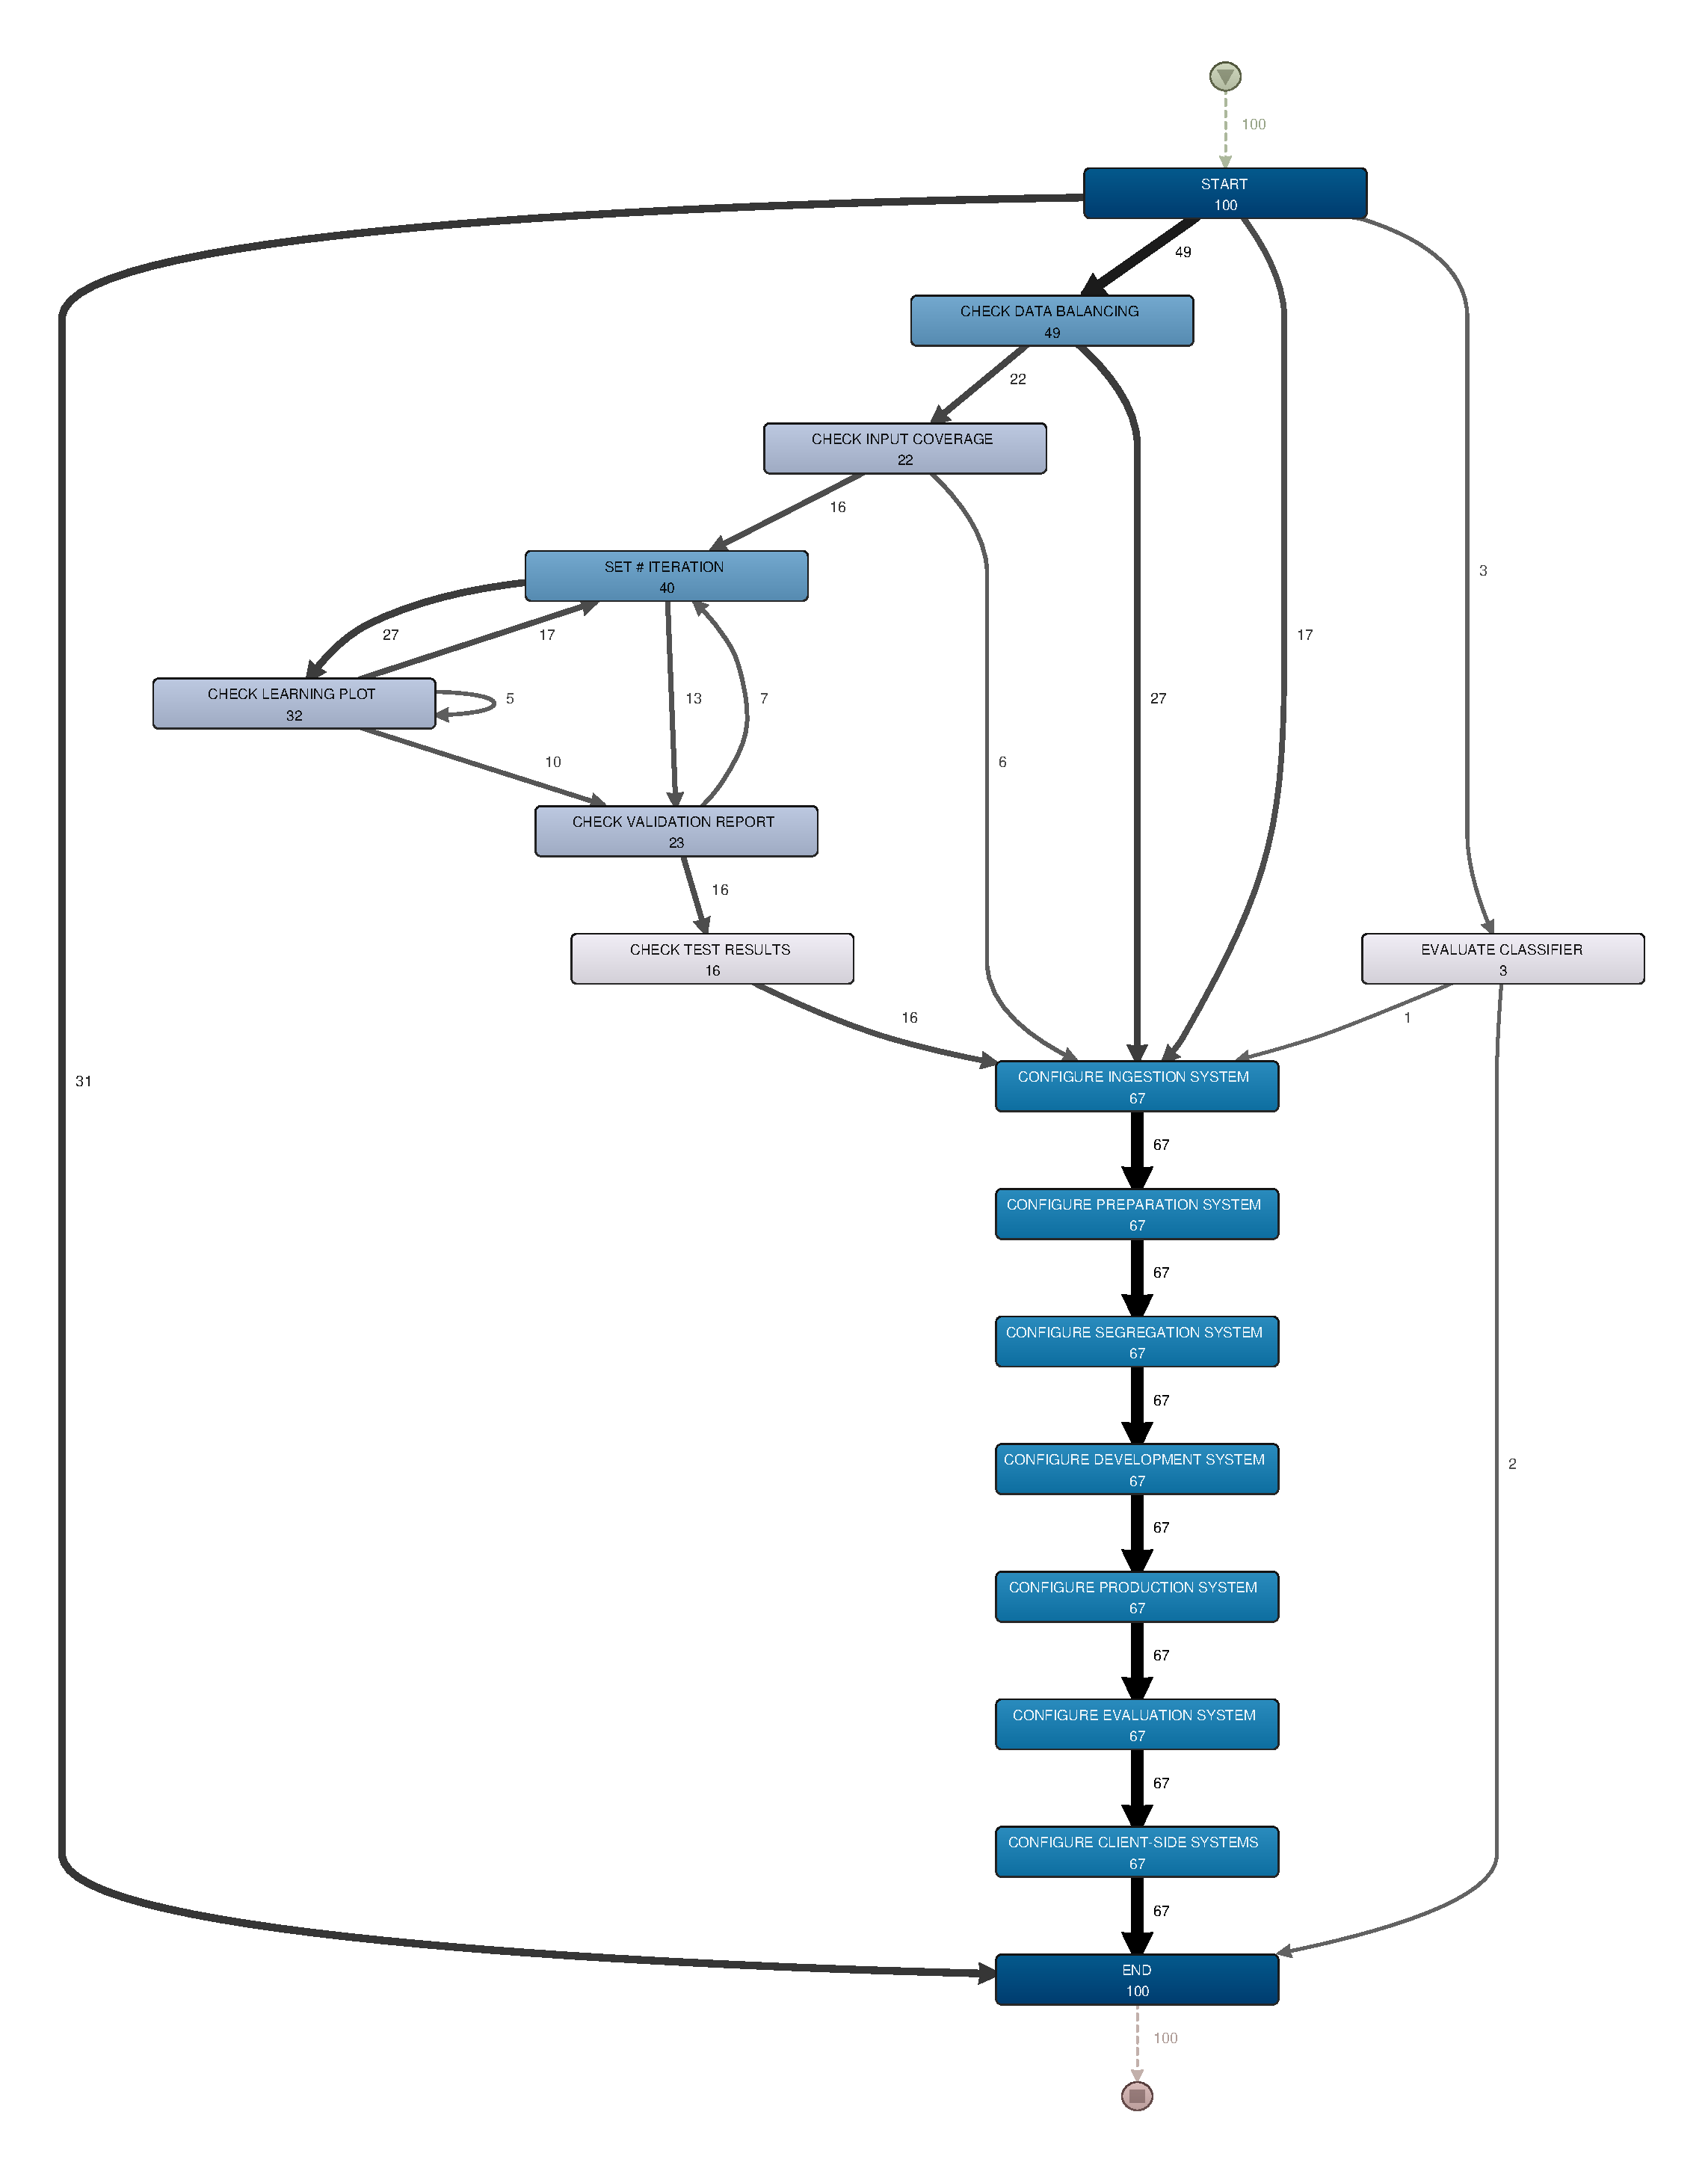
\includegraphics[width=0.8\textwidth]{figures/disco_map.pdf}
\caption{Disco analysis}
\label{fig:disco_analysis}
\end{figure}

\begin{figure}[H]
\centering
\includegraphics[width=\textwidth]{figures/apromore_map.pdf}
\caption{Apromore analysis}
\label{fig:apromore_analysis}
\end{figure}

As we can see, the two transition maps mined from Disco and from 
Apromore are identical. The only difference stays in the frequencies
because in Disco the frequencies are calculated as the total number of
times a transition is executed, even on the same token; while in Apromore
the frequencies are calculated as the number of individual tokens that execute a
transition. This behavior can be changed with a setting in both tools.

\begin{figure}[H]
\centering
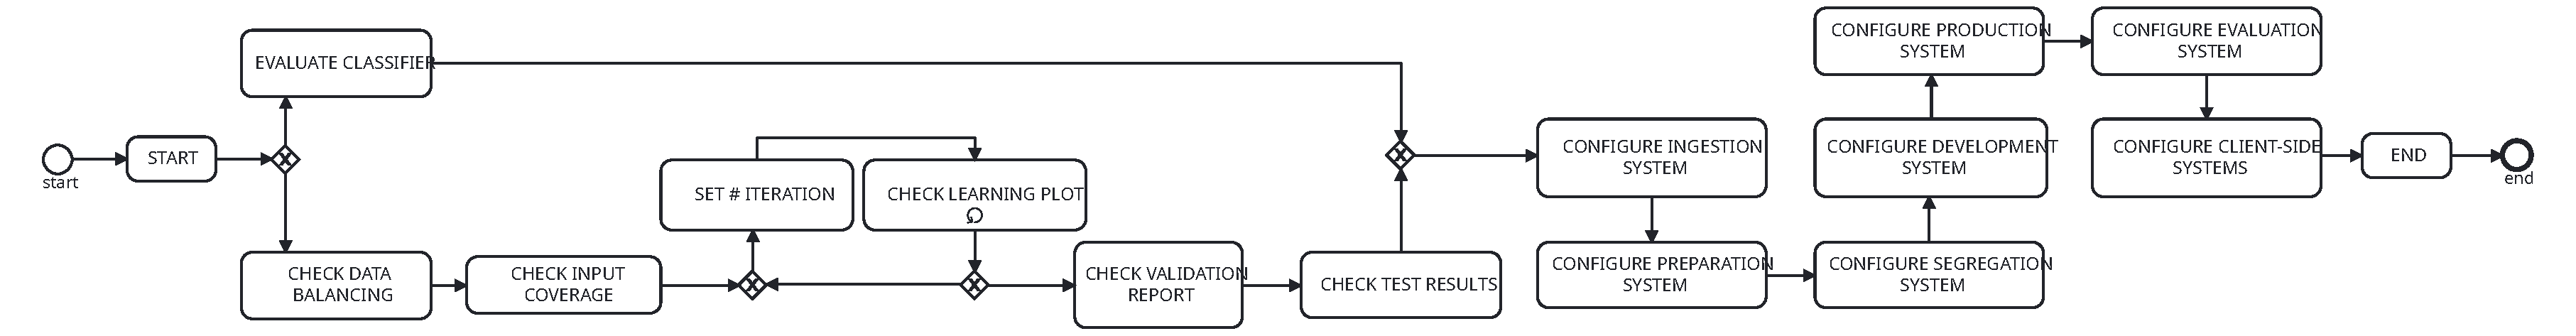
\includegraphics[width=\textwidth]{figures/prom_mined.pdf}
\caption{ProM mined BPMN model}
\label{fig:prom_mined}
\end{figure}

We mined the logs using the "Heuristics Miner ProM6" mining algorithm.

\begin{figure}[H]
\centering
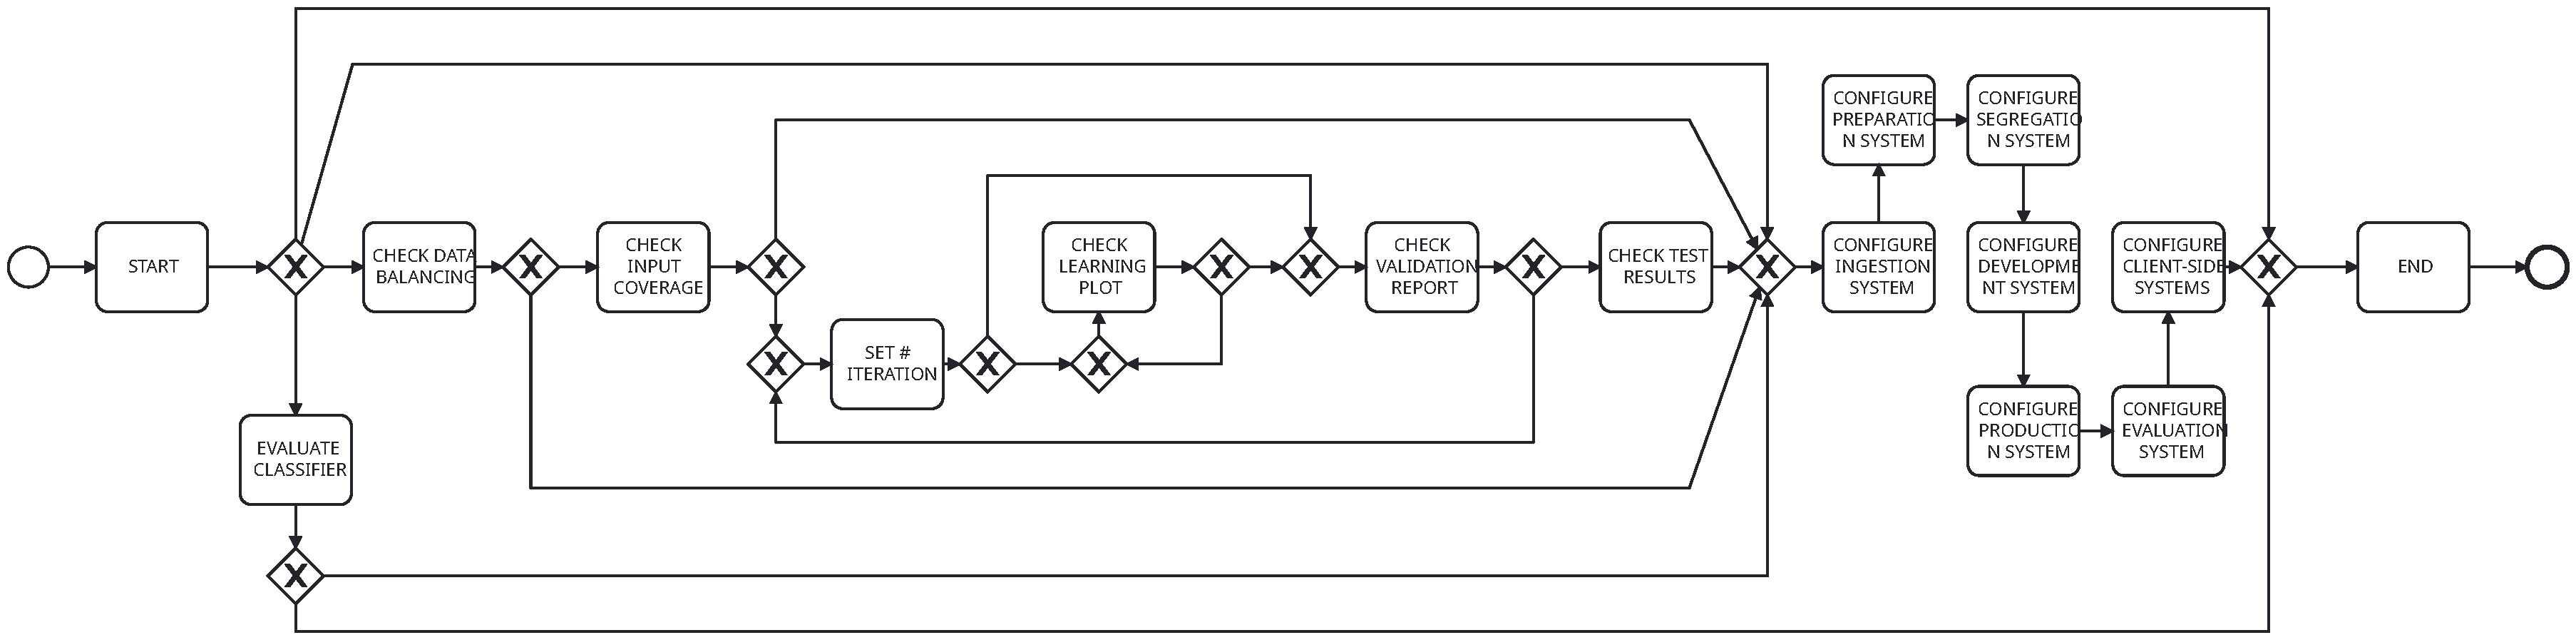
\includegraphics[width=\textwidth]{figures/apromore_mined.pdf}
\caption{Apromore mined BPMN model}
\label{fig:apromore_mined}
\end{figure}

The BPMN model mined from Apromore is more detailed and
covers more cases than the one mined from ProM.
The key differences between the ProM model and the Apromore one are that the
ProM model is missing the paths that skip
the training and the configuration as well as one of the two paths that skip only
the training. Furthermore, the training loop is much simpler in the ProM model, as
it is missing every path that restarts the training after
"CHECK VALIDATION REPORT".

\begin{table}[H]
\centering
\begin{tabular}{|r|l|l|l|l|}
\hline
\textbf{Tool} & \textbf{Fitness} & \textbf{Generalization} & \textbf{Precision} & \textbf{Simplicity} \\
\hline
Apromore & 0.9928 & 0.9837 & 0.8199 & 62 \\
\hline
ProM & 0.7313 & 0.9902 & 0.8653 & 39 \\
\hline
\end{tabular}
\caption{Comparison of the process mining tools}
\label{tab:process_mining_comparison}
\end{table}

\subsection{Violations}
\label{sec:mining_violations}

We modified the logs to introduce 3 violations in the workflow. The
violations are the following:
\begin{enumerate}
    \item Skipping the dataset creation ("CHECK DATA BALANCING"
        and "CHECK INPUT COVERAGE") using data from another user.
    \item Skipping "SET \# ITERATIONS" and "CHECK LEARNING PLOT" by
        using early stopping.
    \item Skipping "CHECK DATA BALANCING" by using a resampling
        technique.
\end{enumerate}

Each violation is introduced 3 times in the logs.

These 3 violations can be beneficial in terms of time and resources:
\begin{itemize}
    \item The first violation can make the costs of the training significantly
    lower for the client, because using an old dataset allows us to skip 
    the labeling of the new data and it usually is very expensive. 
    Also the manual check of the dataset is skipped saving additional time and
    resources. It must be noted that this violation can be a problem for
    the privacy of the clients and also result in worse models if the data of
    the new user has different characteristics from the old one.
    \item The second violation can make the training faster, because we do not
    need anymore to check the learning plot manually and we can train each
    model only once instead of trying multiple times with different number of
    iterations. Also, the method previously used to determine the number of
    iterations was based on an heuristic and it can be prone to errors.
    \item The third violation can reduce the time and costs of the dataset
    creation, also making the training possible with unbalanced datasets.
\end{itemize}

\begin{table}[H]
\centering
\begin{tabular}{|r|l|l|l|}
\hline
\textbf{CaseID} & \textbf{Violation} & \textbf{Fitness ProM} & \textbf{Fitness Apromore} \\
\hline
10 & 1 & 0.91 & 0.87 \\
\hline
20 & 1 & 0.85 & 0.84 \\
\hline
47 & 1 & 0.86 & 0.86 \\
\hline
53 & 2 & 0.91 & 0.93 \\
\hline
63 & 2 & 0.84 & 0.82 \\
\hline
88 & 2 & 0.91 & 0.93 \\
\hline
6 & 3 & 0.91 & 0.93 \\
\hline
72 & 3 & 0.91 & 0.85 \\
\hline
81 & 3 & 0.94 & 0.87 \\
\hline
\end{tabular}
\caption{Cases, violations and fitness on models generated by ProM and Apromore}
\label{tab:violations}
\end{table}

\begin{table}[H]
\centering
\begin{tabular}{|r|l|}
\hline
\textbf{Tool} & \textbf{Fitness} \\
\hline
Apromore & 0.9875 \\
\hline
ProM & 0.7256 \\
\hline
\end{tabular}
\caption{New fitness with violations included in the logs}
\label{tab:violations_fitness}
\end{table}

\begin{figure}[H]
\centering
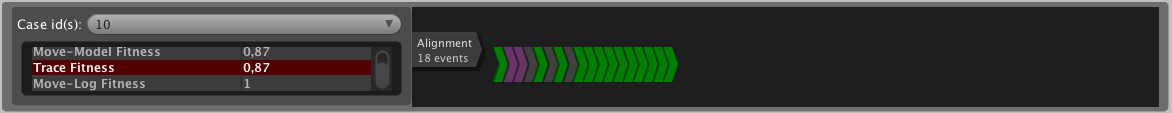
\includegraphics[width=0.8\textwidth]{figures/violation_case/10-apromore.png}
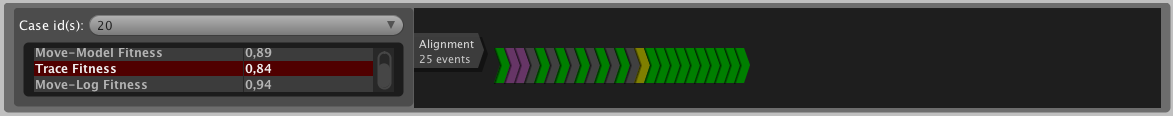
\includegraphics[width=0.8\textwidth]{figures/violation_case/20-apromore.png}
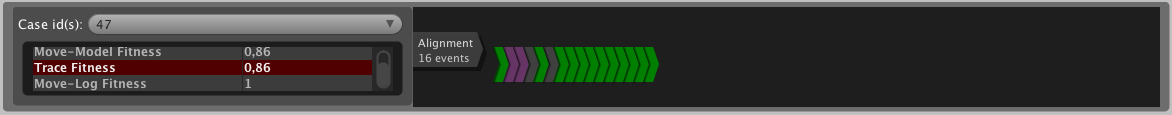
\includegraphics[width=0.8\textwidth]{figures/violation_case/47-apromore.png}

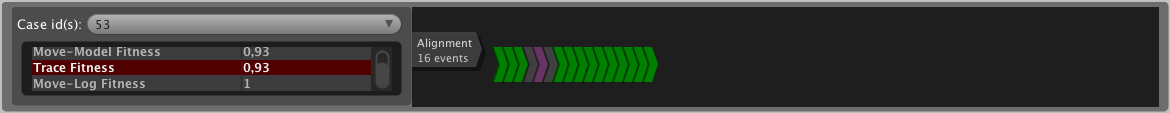
\includegraphics[width=0.8\textwidth]{figures/violation_case/53-apromore.png}
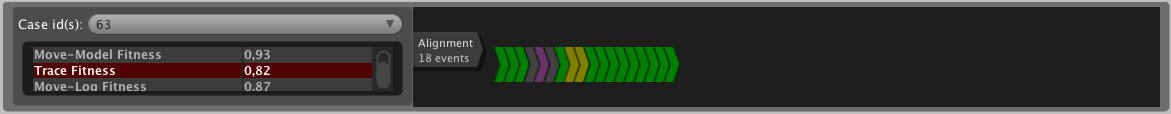
\includegraphics[width=0.8\textwidth]{figures/violation_case/63-apromore.png}
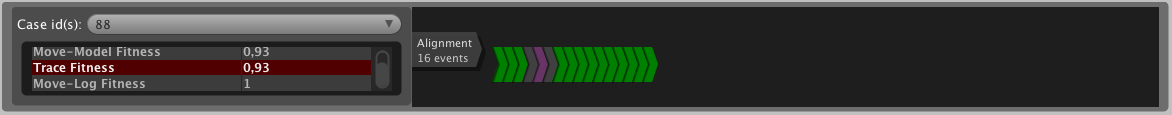
\includegraphics[width=0.8\textwidth]{figures/violation_case/88-apromore.png}

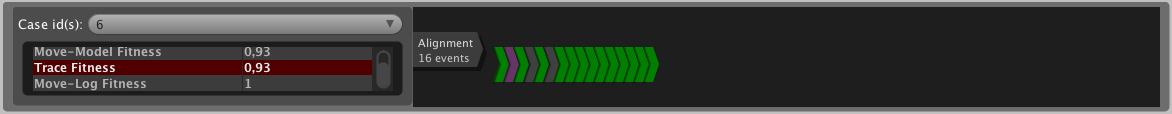
\includegraphics[width=0.8\textwidth]{figures/violation_case/6-apromore.png}
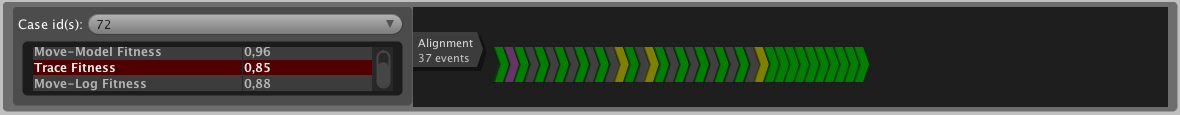
\includegraphics[width=0.8\textwidth]{figures/violation_case/72-apromore.png}
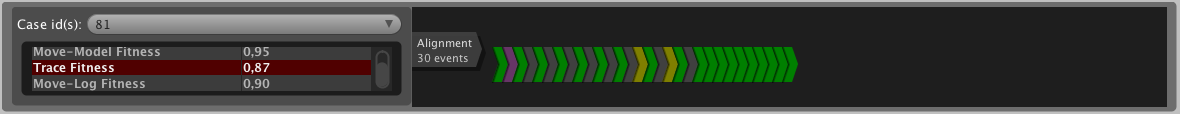
\includegraphics[width=0.8\textwidth]{figures/violation_case/81-apromore.png}
\caption{Violations in the Apromore model visualized with ProM}
\label{fig:violations_apromore}
\end{figure}

\begin{figure}[H]
\centering
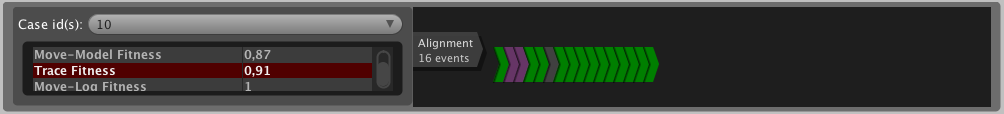
\includegraphics[width=0.8\textwidth]{figures/violation_case/10-prom.png}
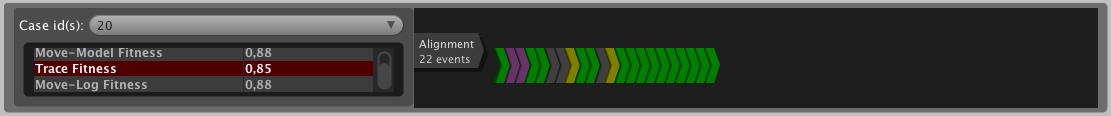
\includegraphics[width=0.8\textwidth]{figures/violation_case/20-prom.png}
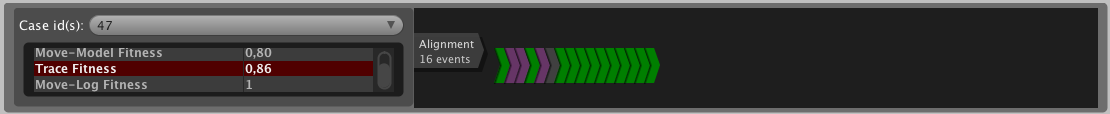
\includegraphics[width=0.8\textwidth]{figures/violation_case/47-prom.png}

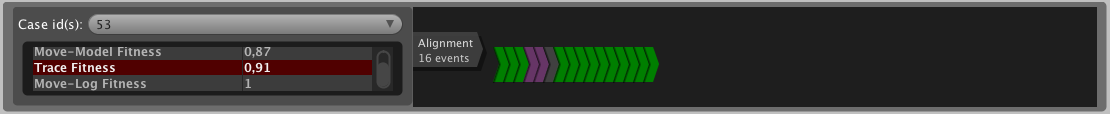
\includegraphics[width=0.8\textwidth]{figures/violation_case/53-prom.png}
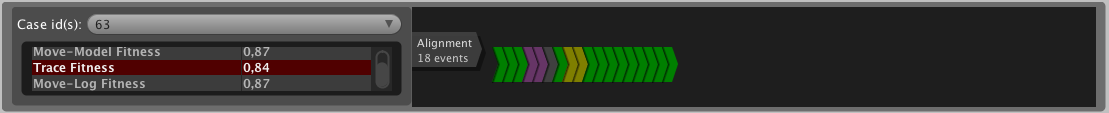
\includegraphics[width=0.8\textwidth]{figures/violation_case/63-prom.png}
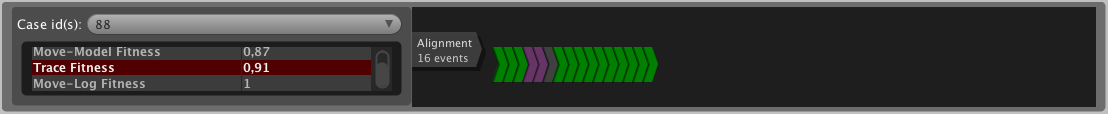
\includegraphics[width=0.8\textwidth]{figures/violation_case/88-prom.png}

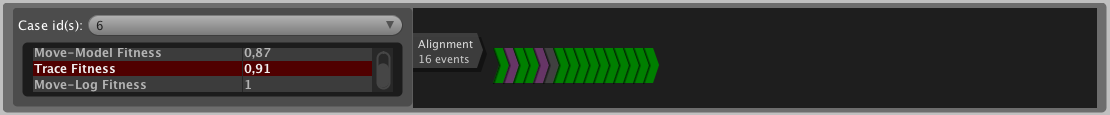
\includegraphics[width=0.8\textwidth]{figures/violation_case/6-prom.png}
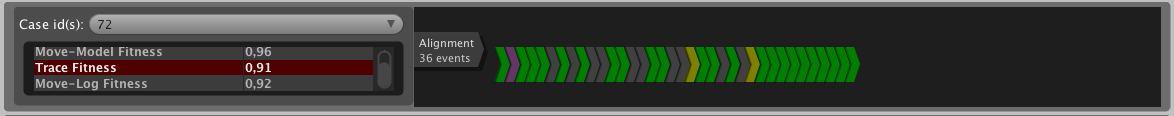
\includegraphics[width=0.8\textwidth]{figures/violation_case/72-prom.png}
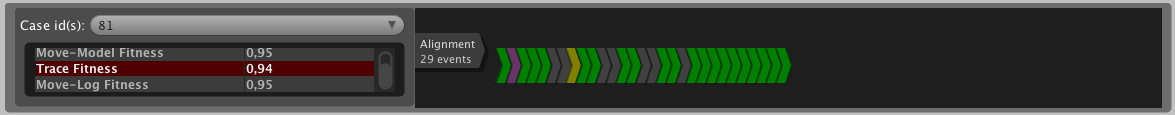
\includegraphics[width=0.8\textwidth]{figures/violation_case/81-prom.png}
\caption{Violations in the ProM model visualized with ProM}
\label{fig:violations_prom}
\end{figure}
